
\section{\textcolor{black}{UQ framework}}
%------------------------------------------------
% \begin{frame}
% \frametitle{Experiments, Models, Simulations, and UQ}
% \begin{figure}
% 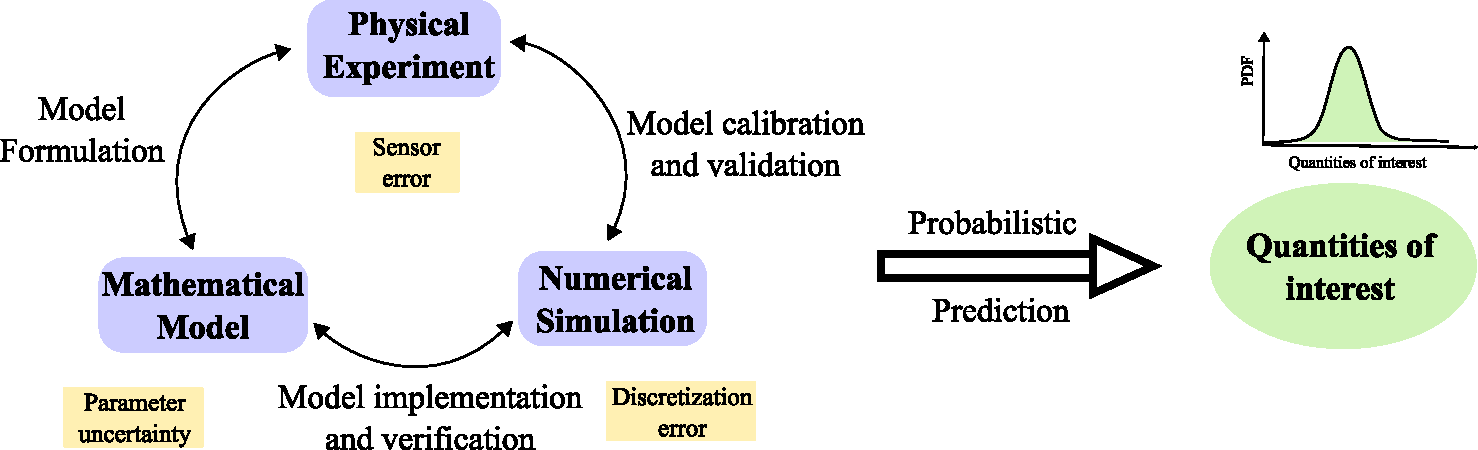
\includegraphics[scale=0.6]{figures/figure-UQ_physics_Model_Simulation.pdf}
% \end{figure}
% \end{frame}

%------------------------------------------------
\begin{frame}
\textbf{\frametitle{UQ framework and components}
\only<1>{
\begin{figure}
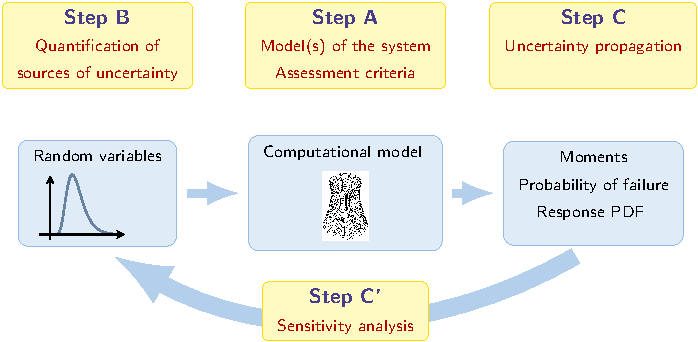
\includegraphics[scale=0.9]{figures/figure-UQ_components_bruno.pdf}
\tiny\footcite{sudret2018}
\end{figure}}
}
\only<2>{
Two UQ types of problems:
\begin{figure}
\centering
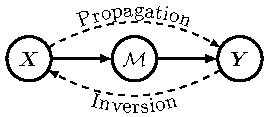
\includegraphics[width=6.5cm]{figures/figure_UQ_propagation_inversion.pdf}
\end{figure}  
\begin{block}{Four components:}
\begin{enumerate}
    \item Model assessment
    \item Uncertainty propagation
    \item Model calibration
    \item Sensitivity analysis
\end{enumerate}  
\end{block}
  


}

\end{frame}

%------------------------------------------------
\begin{frame}
\frametitle{UQ component one: Model assessment}
\begin{definition}
  A computational model $\mathcal{M}$ should contain:
    \begin{itemize}
        \item a \alert{mathematical description} of the physics 
        \item may be seen as a \alert{black box} to compute the QoI
    \end{itemize}
\end{definition}

\bigskip
\begin{itemize}
    \item Analytical formula 
    \item Empirical formula 
    \item Packaged programs based on FEM/FDM ...
    \item $\cdots$
\end{itemize}

\end{frame}

%------------------------------------------------------------------------------------------------------------------------
\begin{frame}
 \frametitle{UQ component one: Model assessment}
 \begin{figure}
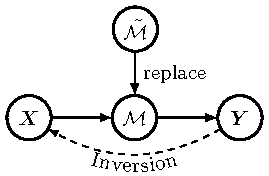
\includegraphics[width=5cm]{figures/figure-surrogate_GraphicalNode.pdf}
\end{figure} 
\only<1>{\begin{itemize}
\begin{block}{Usage}
\centering
$\mathcal{M}(\boldsymbol{x})  \ \ \ \ \approx  \ \ \ \ \tilde{\mathcal{M}}(\boldsymbol{x})$\\
\alert{Hours to run}  \ \ \ \ \ \ \textcolor{green}{seconds to run}
\end{block}
    \item It is built from a \alert{limited} set of runs of the original model $\mathcal{M}$ called the \alert{experimental design} $\mathcal{X} = \{\boldsymbol{x}^{(i))},i=1,\cdots,N\}$
    \item It assume some regularity of the model $\mathcal{M}$ and some general functional shape
\end{itemize}}
\only<2>{
Some popular choices for $\tilde{\mathcal{M}}$:
\begin{table}
\small
\begin{tabular}{lll}
\hline
Name                              & \multicolumn{1}{c}{Shape} & \multicolumn{1}{c}{Parameters} \\ \hline
\alert{Polynomial chaos expansions}       &                           $\tilde{\mathcal{M}}(\boldsymbol{x})
=
\sum_{\boldsymbol{\alpha} \in \mathcal{A} } 
\boldsymbol{y_{\alpha}} \Psi_{\boldsymbol{\alpha}} (\boldsymbol{x})$&                                $\boldsymbol{y_{\alpha}}$\\
Low-rank tensor approximations    &                           $\tilde{\mathcal{M}}(\boldsymbol{x})
=
\sum_{l=1}^{R} b_{l}
\left ( 
\prod_{i=1}^{M}  v_{l}^{i}x_{i}
 \right ) 
$&                                $b_{l}, \  z_{k,l}^{i}$\\
Kriging (a.k.a Gaussian processs) &                           $\tilde{\mathcal{M}}(\boldsymbol{x})
=
\boldsymbol{\beta}^{T} \cdot \boldsymbol{f}(\boldsymbol{x})
 + Z(\boldsymbol{x},\omega)$&                                $\boldsymbol{\beta}, \ \sigma_{Z}^{2}, \  \boldsymbol{\theta}$\\
Support vector machines           &                           $\tilde{\mathcal{M}}(\boldsymbol{x})
=
\sum_{i=1}^{m}
a_{i} K(\boldsymbol{x}_{i},\boldsymbol{x}) 
+b$&                                $\boldsymbol{a}, \ b$\\
Neural networks                   &                           $\tilde{\mathcal{M}}(\boldsymbol{x})
=
f_{n}\left ( 
\cdots f_{2}(
b_{2} + f_{1}(
b_{1} + \boldsymbol{w}_{1} \cdot \boldsymbol{x}
)
\cdot \boldsymbol{w}_{2}
)
\right ) $&                                $\boldsymbol{w}, \ \boldsymbol{b}$\\ \hline
\end{tabular}
\end{table}}
\end{frame}




%-----------------------------------------------------------------------------------------------------------------------
 %---------------------------------------------------------------------------------------------------
\begin{frame}
 \frametitle{UQ component two: Model calibration}
 \only<1>{
 \framesubtitle{Choice for UQ inversion}
\begin{columns}
    \column{0.5\textwidth}
        Choice for the UQ method is totally based on the {\textcolor{red}{\textbf{quantity}}} of accessible data:
        \begin{itemize}
            \item  {\textcolor{red}{\textbf{Lack}}} or {\textcolor{red}{\textbf{no}}} data available, model can be solely based on expert judgement
            \item {\textcolor{red}{\textbf{Substantial}}} volume data available, model can fully use statistical inference (e.g., the methods of moments)
            \item {\textcolor{red}{\textbf{Combination}}} of two above: Bayesian methods
            \begin{equation*}           \pi(\boldsymbol{x}|\mathcal{Y}) = \frac{{\mathcal{L}(\boldsymbol{x}|\mathcal{Y}) \cdot \pi(\boldsymbol{x})}}{{\pi(\mathcal{Y})}} 
            \end{equation*}
        \end{itemize}
    
    \column{0.5\textwidth}
        \begin{figure}[!ht]      
        %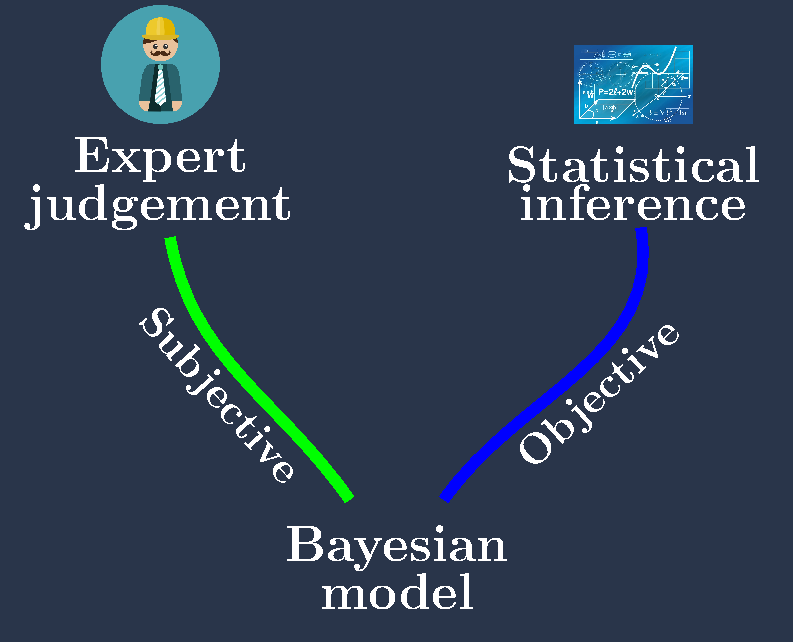
\includegraphics[scale=0.6]{figures/figure_objvssub.pdf}
        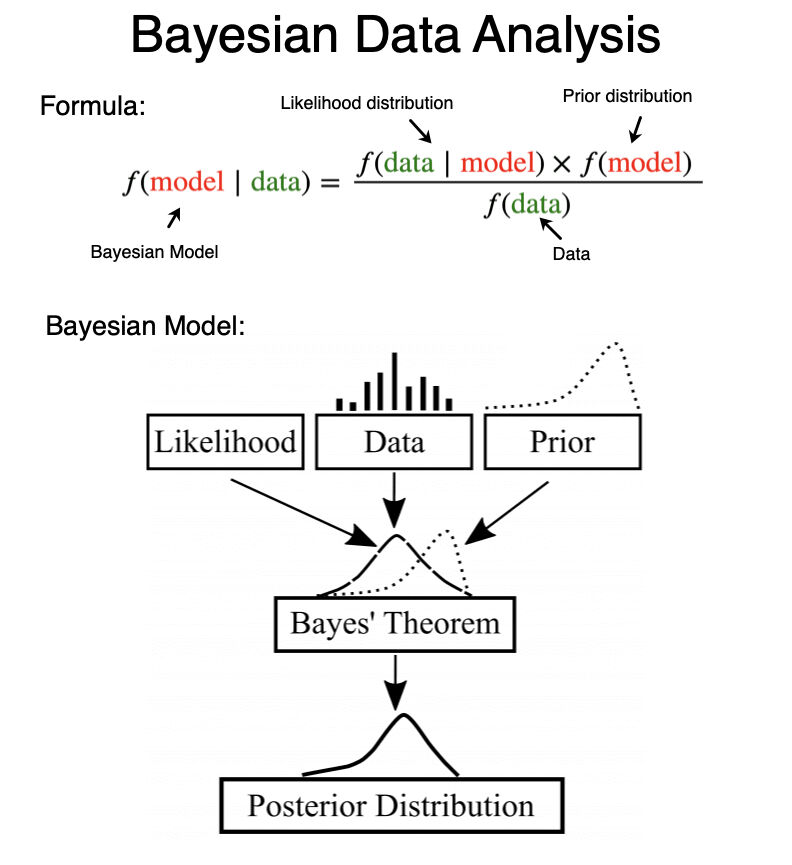
\includegraphics[scale=0.20]{figures/figure_Bayesflow.jpg}        \end{figure}\tiny\footnotetext{\href{https://en.wikipedia.org/wiki/Weather_Research_and_Forecasting_Model}{From Matt Dancho}}
\end{columns}
 }


\only<2>{
\begin{block}{Bayesian methods}
    Expert guess + Limited data $\rightarrow$ Distribution
\end{block} 
\begin{columns}
    \column{0.5\textwidth}
    Prior:
    \begin{figure}[!ht]       
    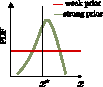
\includegraphics[scale=2.2]{figures/figure-weakandstrongprior.pdf}
    \end{figure}
    
    \column{0.5\textwidth}
    Likelihood:
    \begin{figure}[!ht]       
    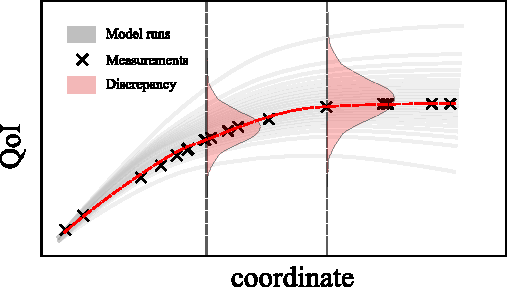
\includegraphics[scale=2.7]{figures/figure-likelihood.pdf}
    \end{figure} 
\end{columns}
\begin{alertblock}{Notable caveats:}

\begin{itemize}
    \item Prior-Requires specific expertise 
    \item Likelihood-Computationally expensive 
\end{itemize}  
\end{alertblock}
}



 \end{frame}
 %======================================================================================================
%--------------------------------------------------------------------------------------------

\begin{frame}
 \frametitle{UQ component three: Uncertainty propagation}
 
 \only<1>{
 \begin{figure}
    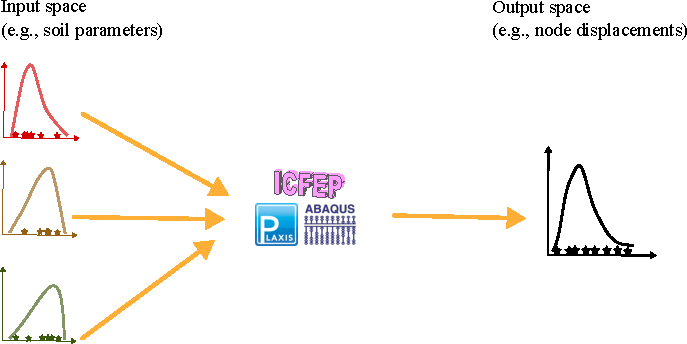
\includegraphics[scale=0.9]{figures/figure-UQ_propagation_MC.pdf}
\end{figure}
\begin{itemize}
\setlength\itemsep{0.5cm}
\item \alert{Output statistics}, i.e., mean, standard deviation. etc.
\begin{equation*}
    \mu_{\boldsymbol{Y}} = \mathbb{E}_{\boldsymbol{X}}
[\mathcal{M}(\boldsymbol{X}) ]; \ 
\sigma^2_{\boldsymbol{Y}} = \mathbb{E}_{\boldsymbol{X}}
[(\mathcal{M}(\boldsymbol{X}) - \mu_{\boldsymbol{Y}})^2]
\end{equation*}
\item \alert{Distribution} of the QoI
\item \alert{Probability} of exceeding an admissible threshold $y_{adm}$ following $P_{f} = \mathbb{P}(\boldsymbol{Y} \ge y_{adm})$
\end{itemize}
 }



 \end{frame}

 %---------------------------------------------------------------------------------------------------
\begin{frame}
 \frametitle{UQ component four: Sensitivity analysis}

  
 \only<1>{
 \begin{quote}
   \Large Sensitivity analysis-Determine what are the input parameters whose uncertainty explains the variability of the QoI   
 \end{quote}{}


\begin{columns}
    \column{0.5\textwidth}
    \begin{itemize}
        \item detect input parameters whose uncertainty has \alert{no impact} on the output variability
        \item detect input parameters which allow one to best \alert{decrease the output variability} when set to a deterministic value
        \item detect \alert{interactions} between parameters
    \end{itemize}
    \column{0.5\textwidth}
\begin{figure}          
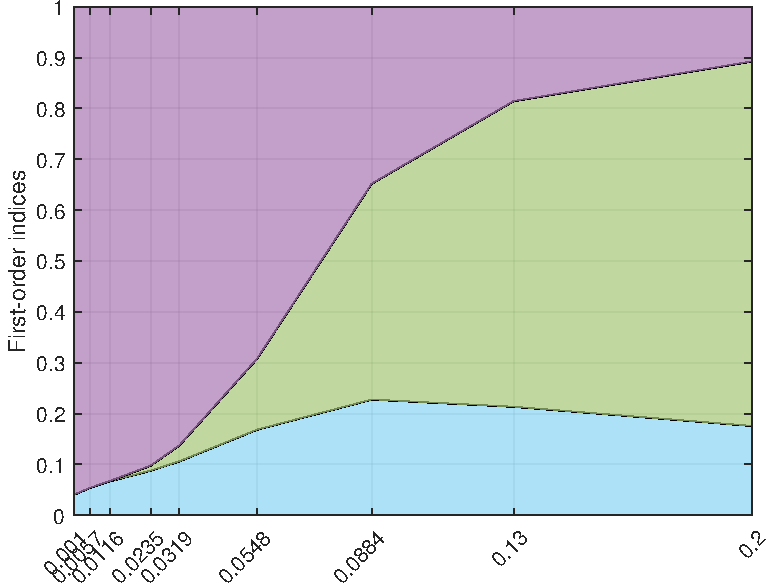
\includegraphics[scale=1.3]{figures/figure-Sobol.pdf}
\tiny\footfullcite{sudret2018}
\end{figure}
\end{columns}
 }

\only<2>{
\begin{block}{Total variance:}
\begin{equation*}
D\equiv \text{Var}[\mathcal{M}(\boldsymbol{X}) ]
= \text{Var}[\sum_{u \subset \{1,\cdots,M\}} \mathcal{M}_{u}(\boldsymbol{X}_{u}) ]
= \sum_{u \subset \{1,\cdots,M\}} \text{Var}[\mathcal{M}_{u}(\boldsymbol{X}_{u}) ] 
\end{equation*}    
\end{block}

\begin{itemize}
    \item Sobol's indice:
    \begin{equation*}
S_u   \overset{\mathrm{def}}{=} \frac{\text{Var}[\mathcal{M}_{u}(\boldsymbol{X}_{u}) ] }{D} 
    \end{equation*}

    \item First-order Sobol's indice:
     \begin{equation*}
S_i = \frac{D_i}{D} = \frac{\text{Var}[\mathcal{M}_{i}(\boldsymbol{X}_{i}) ] }{D}
    \end{equation*}
    Quantify the effect of each input parameter \alert{separately}

    \item Total Sobol's indice:
    \begin{equation*}
S_{i}^{T} \overset{\mathrm{def}}{=}  
\sum_{u \supset i} S_u
    \end{equation*}
    Quantify the \alert{total effect} of $x_{i}$, including \alert{interactions} with other variables
\end{itemize}
}

 \end{frame}
 %--------------------------------------------------------------

 
\begin{frame}
\frametitle{Uncertainty quantification for engineering problems}
Research topics
\begin{itemize}
    \item \textcolor{red}{Uncertainty modelling for engineering systems}
    \item \textcolor{red}{Bayesian model calibration}
    \item Structural reliability analysis
    \item Surrogate models (low dimensions/high dimensions)
    \item Stochastic inverse problem
    \item Global sensitivity analysis
    \item Reliability-based design optimization
    \item ...
\end{itemize}

\end{frame}




